{\color{red}

  \section{On correlated systematic uncertainties}
  \label{app:corr}

As discussed in Sect.~\ref{sec:MCreplicas}, in this work
we assume that the uncertainties associated to the measured
bin-by-bin spectra are uncorrelated among them.
%
However, in general we know that there could be systematic effects,
for instance of instrumental origin, which might induce
a pattern of correlated systematic uncertainties in the training
data.
%
Should this information be available, one can then
account for it through the Monte Carlo replica
generation by using Eq.~(\ref{eq:MCreplicaGen}) rather than
Eq.~(\ref{eq:MCreplicaGen2}), and likewise
Eq.~(\ref{eq:chi2}) can be augmented such that the likelihood
function used for the ML training
is based on the full experimental covariance matrix,
rather than on only of its diagonal component.

%%%%%%%%%%%%%%%%%%%%%%%%%%%%%%%%%%%%%%%%%%%%%%%%%%%%%%%%%%%%%%%%%%%%%%%
\begin{figure}[t]
\begin{centering}
  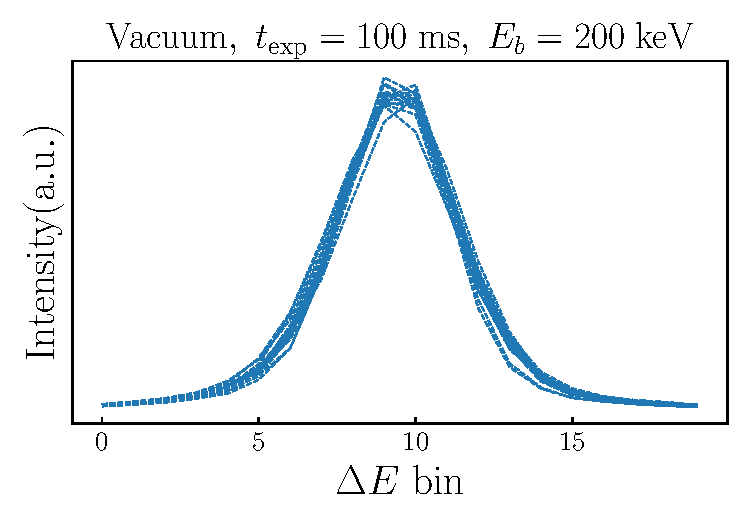
\includegraphics[width=0.80\linewidth]{plots/spectra-app.pdf}
  \caption{\small \color{red} The EELS intensities associated
    to the $N_{\rm sp}=15$ individual vacuum spectra, after the discretization
    procedure, listed as "Set 1"
    in Table~\ref{table:vacuumdata}.
    %
    These spectra have been acquired under nominally
    identical operation conditions 
    corresponding to $t_{\rm exp}=100$ ms and $E_b=200$ KeV.
    %
    In the $x$ axis, the number of the $\Delta E$ bin is displayed.
  }
\label{fig:spectra-app}
\end{centering}
\end{figure}
%%%%%%%%%%%%%%%%%%%%%%%%%%%%%%%%%%%%%%%%%%%%%%%%%%%%%%%%%%%%%%%%%%%%%%%%%%


While it is beyond the scope of this work to
assess the possible presence of correlated systematic
errors in our training dataset, we present here a first
investigation of the correlation patterns present.
%
To this end, one can evaluate the correlation coefficient
between two bins in the electron energy loss $\Delta E$, that is
defined as
 \be
\label{eq:corriexp}
\rho_{ij}^{\rm (exp)} \equiv \rho(\Delta E_i, \Delta E_j)= \frac{ \frac{1}{N_{\rm sp}} \sum_{l=1}^{N_{\rm sp}}
  \lp I_{{\rm ZLP},i}^{ ({\rm exp}),l} I_{{\rm ZLP},j}^{ ({\rm exp}),l}  \rp 
- \la I_{{\rm ZLP},i}^{ ({\rm exp})}\ra_{N_{\rm sp}} \la I_{{\rm ZLP},j}^{ ({\rm exp})}\ra_{N_{\rm sp}}}{\sigma_i^{\rm (exp)} \sigma_j^{\rm (exp)} } \, ,\,
\ee
and whose value is close to one (minus one) for two bins that are strongly
correlated (anticorrelated).
%
We compute this correlation coefficients on the spectra displayed
in Fig.~\ref{fig:spectra-app}, which correspond to
the EELS intensities associated
to the $N_{\rm sp}=15$ individual vacuum spectra, after the discretization
procedure, listed as ``Set 1"
in Table~\ref{table:vacuumdata}.
%
These spectra have been acquired under nominally
identical operation conditions 
corresponding to $t_{\rm exp}=100$ ms and $E_b=200$ KeV.
%
In the $x$ axis, the number of the $\Delta E$ bin is displayed.


Fig.~\ref{fig:corrmat-app} then displays this correlation coefficient $\rho(\Delta E_i,\Delta E_j)$, Eq.~(\ref{eq:corriexp}), associated
to the $N_{\rm sp}=15$ individual vacuum spectra shown
in Fig.~\ref{fig:spectra-app}, where lighter (darker)
colors indicate a positive (negative) bin-by-bin correlation.
%
Some of these correlations are expected, for instance, neighbouring
bins are correlated by the underlying physical law.
%
However, others
might be related to an instrumental origin,
in particular one can observe that bins
at large, symmetric values of $\Delta E$ appear to exhibit
a relatively strong correlation.
%
Only the latter should then be included as an additional
source of systematic uncertainty in the MC replica generation
and in the $\chi^2$ definition.

%%%%%%%%%%%%%%%%%%%%%%%%%%%%%%%%%%%%%%%%%%%%%%%%%%%%%%%%%%%%%%%%%%%%%%%
\begin{figure}[t]
\begin{centering}
  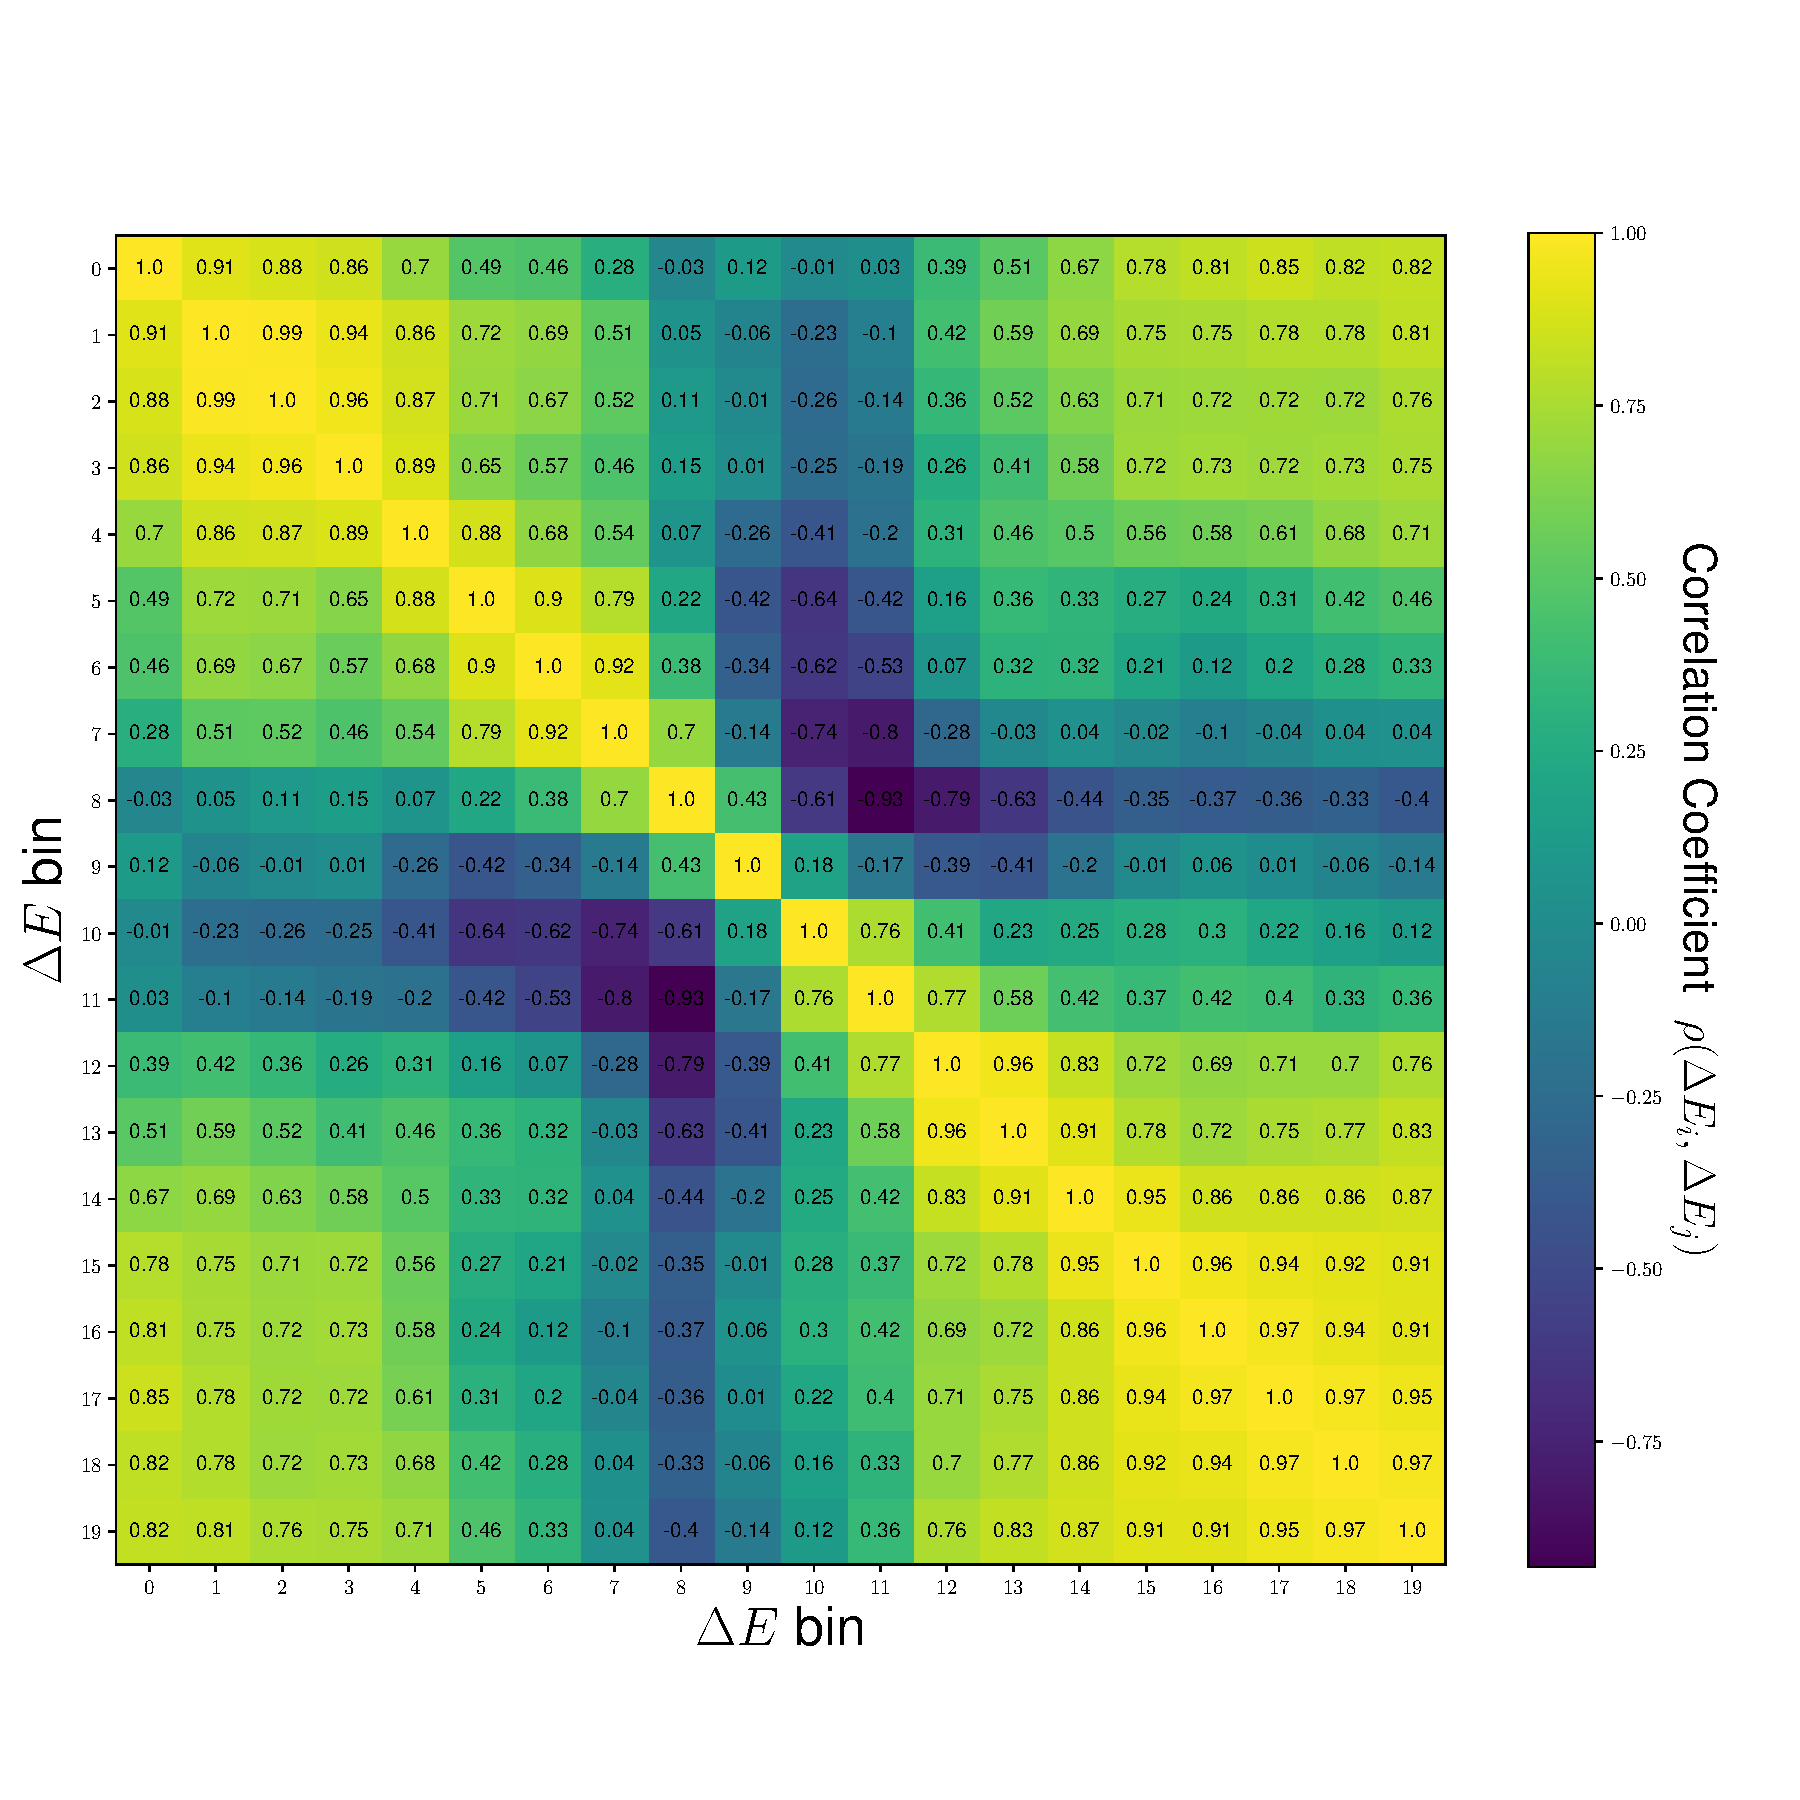
\includegraphics[width=0.92\linewidth]{plots/corrmat-app.pdf}
  \vspace{-0.8cm}
  \caption{\small \color{red} The correlation coefficient $\rho(\Delta E_i,\Delta E_j)$, Eq.~(\ref{eq:corriexp}) associated
    to the $N_{\rm sp}=15$ individual vacuum spectra displayed
    in Fig.~\ref{fig:spectra-app}, where lighter (darker)
    colors indicate a positive (negative) bin-by-bin correlation.
  }
\label{fig:corrmat-app}
\end{centering}
\end{figure}
%%%%%%%%%%%%%%%%%%%%%%%%%%%%%%%%%%%%%%%%%%%%%%%%%%%%%%%%%%%%%%%%%%%%%%%%%%
  
Future work, based on an exhaustive analysis of spectral images,
will provide sufficient information in order to carry out a purely
data-driven determination of the systematic correlated
uncertainties present in our training samples.


  }
